\documentclass[a4paper,12pt,fleqn]{article}%fleqn pour aligner les equations à gauche
\usepackage{../../Styles/Cours}

\newcommand{\chnum}{Chapitre 8}
\newcommand{\chtitle}{Électroraffinage du cuivre}
\newcommand{\dtype}{TP}
  
\begin{document}
	\maketitle

L'industrie de l'hydrométallurgie utilise l'électroraffinage et l'extraction par voie électrolytique de cuivre, de zinc, de nickel, de cobalt, de manganèse et de cadmium. On se propose ici d'étudier l'électroraffinage du cuivre.
\begin{enumerate}
	\item Proposer une définition du mot électroraffinage.
\end{enumerate}

\section{Électrolyse à anode soluble}
	\subsection*{Protocole :}
	\begin{itemize}
		\item Dans un bécher de \SI{100}{mL}, verser \SI{75}{mL} de solution de sulfate de cuivre (II) : $c=\SI{0,5}{\mole\per\liter}$.
		\item Peser la plaque de cuivre décapée : $m(\ce{Cu})_{avant} = ........ \unit{\gram}$
		\item Réaliser le montage schématisé.
		\item Fermer l'interrupteur en déclenchant le chronomètre et maintenir le courant à une intensité $I = \SI{0,10}{A}$ ($U\approx \SI{1,3}{V}$) pendant une quinzaine de minutes.
		\item Sécher l'électrode de cuivre et la peser : $m(\ce{Cu})_{apres} = ........ \unit{\gram}$
		\item Calculer la masse de cuivre déposée $m_{déposée} = ........ \unit{\gram}$
	\end{itemize}
\begin{figure}[h!]
	\caption{\textbf{Schéma du montage}}
	\centering 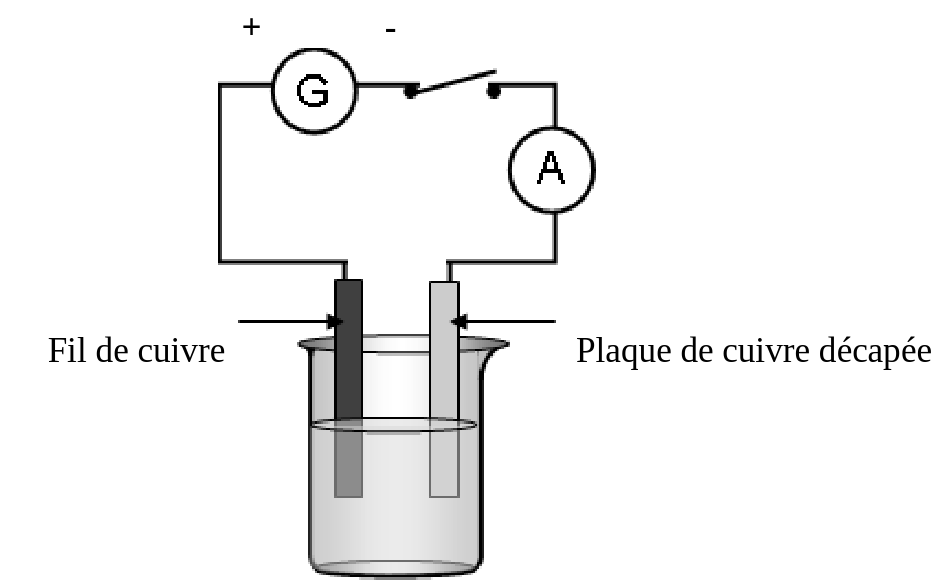
\includegraphics[width=.5\linewidth]{Ressources/TSPE_C16a_Electroraffinage_Fig1.png}
\end{figure}

\begin{enumerate}[resume]
	\item Qu'observe-t-on au niveau des électrodes ?
	\item Pourquoi cette électrolyse est-elle appelée : électrolyse à anode soluble ?
	\item Sur le schéma, indiquer :
		\begin{itemize}
			\item Le sens du courant
			\item Le sens de déplacement des électrons
			\item Le sens de déplacement des cations \ce{Cu^2+}
			\item Le sens de déplacement des anions \ce{SO4^2-}
		\end{itemize}
	\item En rappelant les réactions ayant lieux à l'anode et à la cathode, écrire les deux demi-équations électroniques mises en jeu.
	\item A quelle électrode doit-on mettre le métal brut ?
	\item A quelle électrode récupère-t-on le cuivre métallique ?
	\item Quel est l'intérêt de cette électrolyse ?
	\item Comment varie la concentration en ions cuivre dans la solution ?
\end{enumerate}

\section{Bilan de matière}
\begin{enumerate}[resume]
	\item Déterminer la quantité de matière d'électrons échangés $n_{\ce{e-}}$ pendant l'électrolyse.
	\item Quel est le lien entre la quantité de charge $Q$, l'intensité du courant $I$ et la durée de l'électrolyse $\Delta t$ ?
	\item Quel est le lien entre la quantité de charge $Q$, la quantité de matière d'électrons échangés $n_{\ce{e-}}$ et la constante de Faraday ?
	\item Calculer la masse maximale de cuivre déposé.
	\item Calculer le rendement de l'électrolyse.
\end{enumerate}

\textbf{Données :}
\begin{itemize}
	\item $M(\ce{Cu}) = \SI{63,5}{\gram\per\mole}$
	\item Constante d'Avogadro : $N_A = \SI{6,02E23}{\per\mole}$
	\item Charge élémentaire : $e=\SI{1,60E-19}{C}$
\end{itemize}
\end{document}